\documentclass[a4paper]{article}

\usepackage[T1]{fontenc}
\usepackage[utf8]{inputenc}
\usepackage{graphicx}
\usepackage{fixme}

\usepackage{subcaption}
\usepackage[english, french]{babel}

\usepackage{hyperref}

\usepackage[sorting=ynt, maxnames=10, doi=false, url=false]{biblatex}
\addbibresource{biblio.bib}
\AtEveryBibitem{\clearfield{note}}

\usepackage{palatino}

\newcommand{\eg}{{\textit{e.g.~}}}
\newcommand{\etal}{{\textit{et al.~}}}
\newcommand{\ie}{{\textit{i.e.~}}}

\graphicspath{{figs/}}

\title{Vers le robot cognitif :\\ unifier le signal et le symbole\\ 
    {\large Programme de recherche}}

\author{Séverin Lemaignan}
\date{}

%%% Body
\begin{document}
\maketitle

\begin{figure}
    \centering
    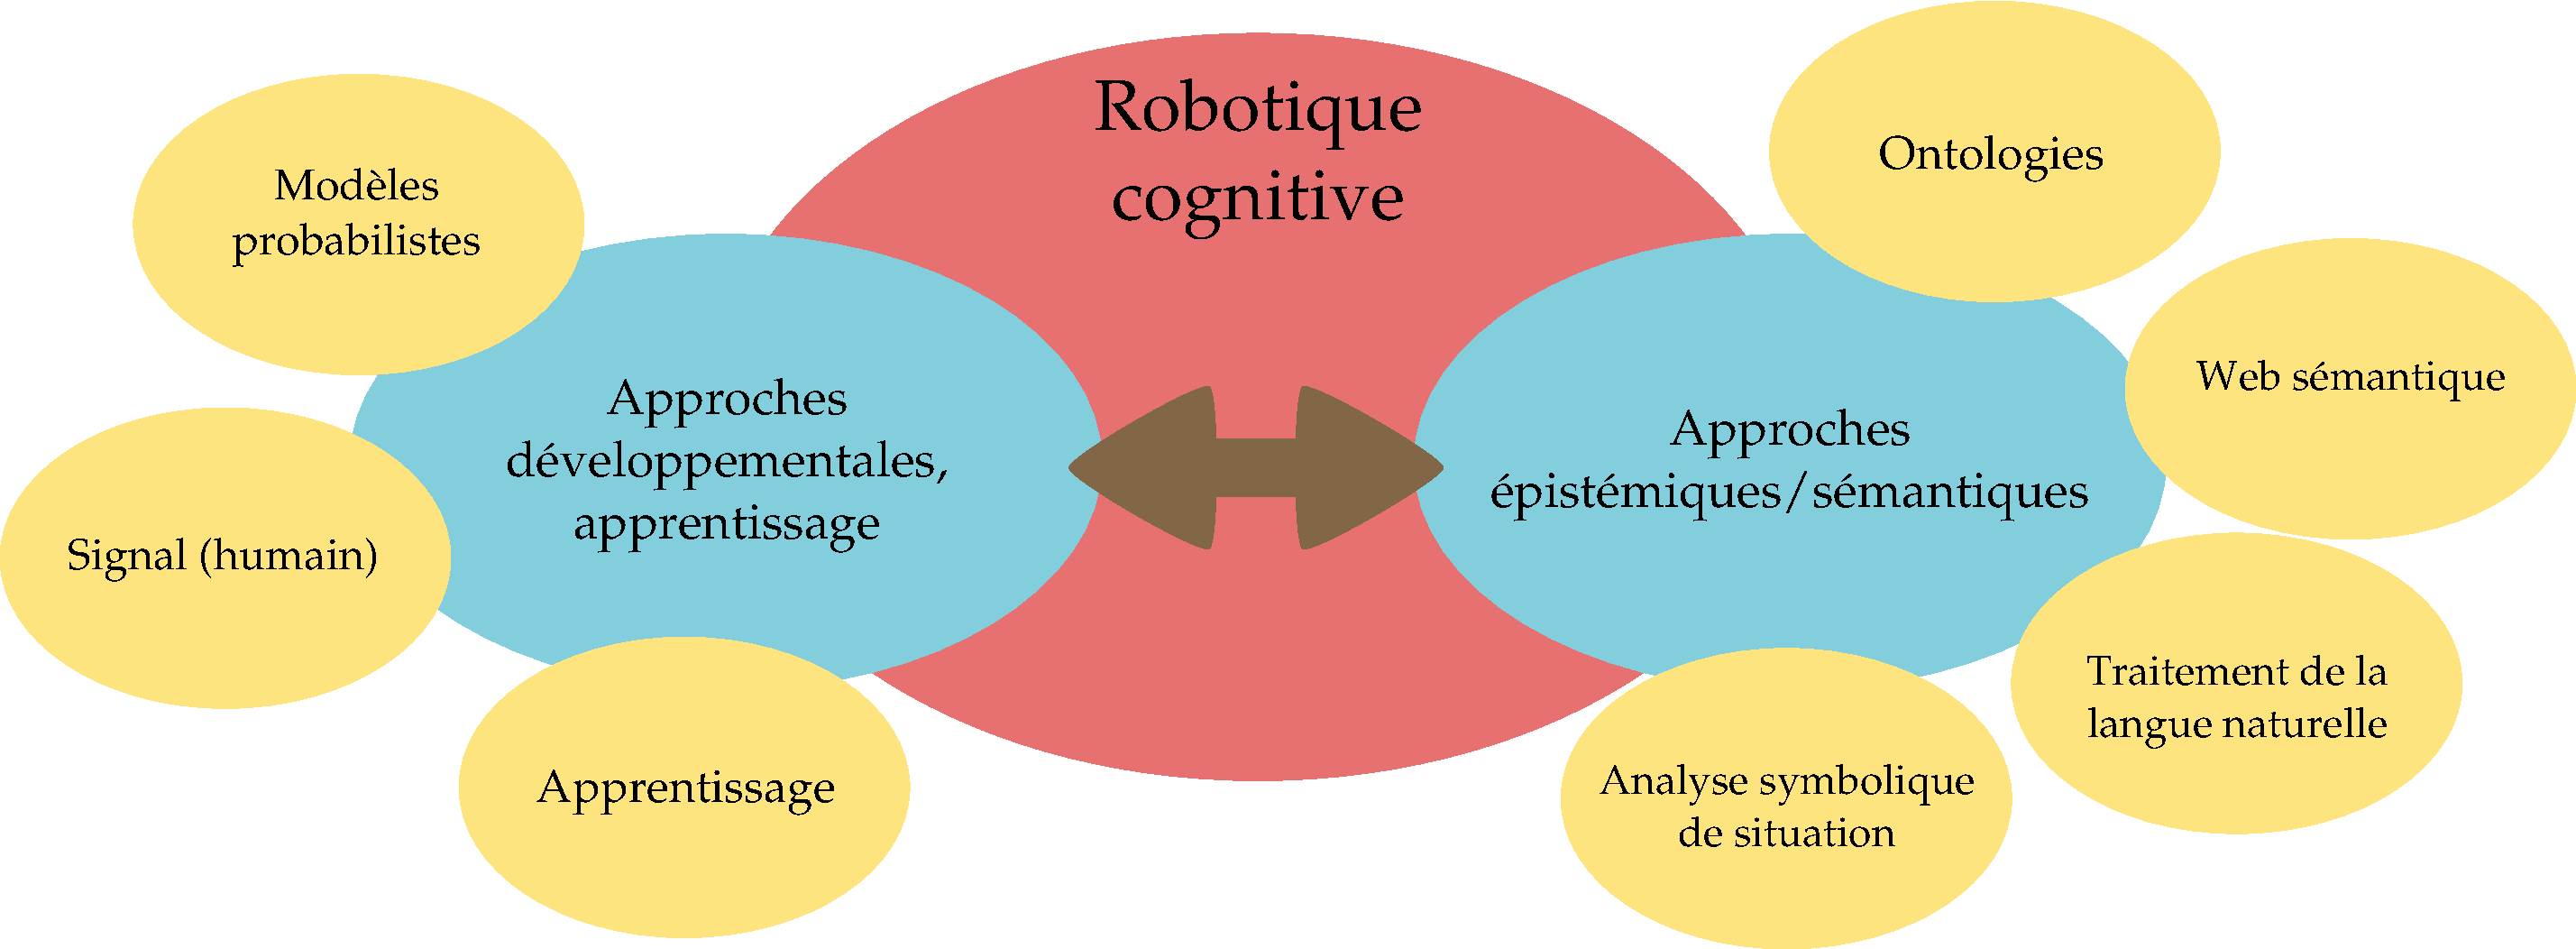
\includegraphics[width=1.0\linewidth]{place}
    \caption{}
    \label{place}
\end{figure}


Deux courants majeurs structurent la recherche en robotique cognitive: les
approches dites épigénétiques (ou développementales, ou encore ancrées) d'une
part, dans lesquelles un certains nombre de mécanismes cognitifs émergent ou
sont appris par le robot au contact de son environnement et de ses interactions
(en particulier avec les humains) ; les approches épistémiques d'autre part,
dans lesquelles les robots manipulent des corpus pré-existants de connaissances,
et qui travaillent avec des concepts essentiellement symboliques et abstraits,
dont la sémantique est explicite.

Mes activités de recherche antérieures se sont focalisées sur les secondes, dans
le cadre particulier de l'interaction homme-robot, qui a l'intérêt d'imposer des
situations riches et complexes d'un point de vue sémantique. Ce choix m'a permis
de mener de premières recherches fructueuses -- sanctionnées par le prix de
thèse du Groupe de Recherche (GdR) Robotique -- tant sur la représentation des
connaissances du robot que sur l'implémentation de capacités cognitives avancées
chez les robots (dans le domaine du langage naturel par exemple). 

Les approches symboliques souffrent cependant d'un manque de polyvalence et
d'adaptibilité. Elles ne sont pas bien adaptées à la représentation des
phénomènes continus ou stochastiques, et ne permettent pas facilement
d'apprendre et de généraliser à partir de situations vécues par le robot. Ce
sont là au contraire les points forts des approches développementales.  Jusqu'à
récemment, ces dernières ont cependant souvent été limitées à des fonctions
cognitives simples. Des efforts récents~\cite{morse2010epigenetic,
pezzulo2012computational} tentent de construire un pont entre les deux
approches, en proposant d'employer la robotique cognitive comme
\emph{méthodologie} pour étudier une cognition ancrée et computationelle. Ces
travaux visent toutefois en premier lieu à mieux comprendre la cognition
\underline{humaine} en employant uniquement le robot comme un support de
modélisation.

Le c\oe ur du projet scientifique que je propose se situe lui aussi au carrefour
de ces deux approches, mais garde une perspective essentiellement robotique :
mon objectif est d'\textbf{accroitre l'autonomie des robots} dans les
environnements particulièrement complexes que sont les environnements humains.
La problématique que je propose de traiter est ainsi comment \textbf{mettre en
place les ponts entre robotique cognitive développementale d'une part et
épistémique d'autre part, afin de faire progresser de manière disruptive la
qualité et la puissance des modèles construits et manipulés par les robots, et
ainsi, leur autonomie}.

Je propose de plus de poser un cadre de recherche précis pour cette
problématique : l'interaction homme-robot. Je veux y appliquer une double
approche, à la fois \emph{bottom-up} en m'intéressant directement au
signal humain émis durant l'interaction, et \emph{top-down} en étudiant
explicitement un certain nombre de tâches cognitives de haut-niveau que le robot
doit pouvoir maitriser, incluant un dialogue multi-modal riche et pertinent ou
encore l'implémentation de formes poussées de théorie de l'esprit.

L'idée maitresse sur laquelle je propose de mener mes recherches est ainsi la
\textbf{combinaison nouvelle de techniques d'apprentissage basées sur les
signaux humains émis durant l'interaction homme-robot et de techniques
symboliques de type ontologies ancrées}. On peut ainsi parler
d'\textbf{ontologies multimodales ancrées}, et à ce titre, ce projet de
recherche se situe au carrefour de la robotique, de la cognition ancrée
(\emph{grounded}) qui inclue les techniques d'apprentissage, et de la cognition
symbolique (figure~\ref{place}).

De manière symétrique, je propose aussi de travailler sur le pendant décisionnel
de cette approche duale cognition ancrée/cognition symbolique en introduisant
une rupture vis-à-vis des approches traditionnelles de type architectures en
couche (contrôle bas-niveau/décision haut-niveau) et architectures
hiérarchiques de type ``subsumption''. L'idée clé est ici de proposer un
\textbf{schéma de décision semi-distribué} où un \textbf{composant cognitif
symbolique orchestre (via des activations et des inhibitions) des boucles
sensori-motrices dites ``réflexes'', construites par apprentissage}.

Mon projet s'articule ainsi en trois axes scientifiques : la recherche de
\textbf{techniques nouvelles permettant de lier signal bas-niveau et modèle
sémantique} ; la conception d'un \textbf{système de représentation unifié,
autour de l'idée d'ontologie multi-modale ancrée} ; la transposition de ces
techniques à la \textbf{décision en robotique, avec la recherche d'une
architecture décisionnelle duale et semi-distribuée}.

Le développement de ces axes est par ailleurs soutenu par \textbf{un programme
expérimental fort}. La menée systématique d'expériences d'interaction en milieux
écologiquement valides reste rare et souvent sujette à des faiblesses
méthodologiques.  Dans la continuité de l'expertise que j'ai acquise en
post-doctorat, je propose d'ancrer et de valider mon travail dans un programme
expérimental ambitieux, qui sache ``sortir du laboratoire'' pour se confronter à
des environnements réalistes et complexes.

\subsection*{Axe 1 -- Du signal humain au modèle sémantique}

Durant une interaction, l'idée de \emph{signal humain} groupe plusieurs
dimensions : la familles des signaux verbaux (parole, dialogue), para-verbaux
(uttérances non verbales) et co-verbaux (gestes accompagnant la parole,
attitudes de la voix), le regard (notamment les mécanismes d'attention
conjointe), la posture, et l'ensemble des gestes déictiques.

Ces dimensions sont essentiellement continues, bruitées, et couvrent un large
spectre de valeurs, avec une variabilité inter-individus élevée. De plus, une
interprétation correcte requiert d'analyser les interactions de ces signaux les
uns avec les autres (en premier lieu, les co-occurences).  Ces caractéristiques
font que le traitement du signal humain se prête particulièrement bien aux
approches s'appuyant sur diverses formes de \emph{machine learning} : le système
apprend à reconnaitre et labéliser de manière automatique des séquences
d'actions dans le flux multi-modal du signal perçu.

Pour autant, l'état de l'art en prise de décision autonome en robotique
s'appuie sur des modèles symboliques abstraits, qui ont le bénéfice de manipuler
une sémantique explicite et de permettre une intégration forte avec les outils
classiques de l'intelligence artificielle (planification de tâche, traitement de
la langue naturelle, etc.).

Le premier défi sur lequel je souhaite travailler est ainsi celui-ci :
concevoir et construire les ponts entre l'état de l'art des techniques d'apprentissage
automatique pour le traitement de signaux (sociaux) complexes, et l'état de
l'art des représentations logiques probabilistes abstraites.

\paragraph{Signal et apprentissage}

L'essentiel des recherches récentes dans ce domaine se sont focalisées sur
l'analyse et la reconnaissance d'épisodes d'interaction en se basant sur des
techniques d'apprentissage automatique de type classification (essentiellement SVM
et Decision Trees) ou modélisation statistique séquentielle (essentiellement
modèles de Markov cachés HMM et réseaux bayésiens dynamiques DBN).

L'un des aspects clés est lié à la labélisation automatique
de situations ou séquences, \ie à l'association automatique de sémantique au
signal. ~\cite{mihoub2014modeling}

[A DEVELOPPER]

\paragraph{Modèles logiques probabilistes}

Intégrer ces modèles probabilistes ancrés dans des mécanismes cognitifs de
haut-niveau, typiquement abstraits, est un corollaire qui a lui aussi fait
l'objet de nombreuses recherches ces dernières années, essentiellement sous la
forme de structures symboliques probabilistes. De Raedt et Kersting donnent un
aperçu général de la question dans~\cite{deraedt2008probabilistic}, et, appliqué
à la robotique, on peut mentionner les réseaux logiques markoviens
MLN~\cite{richardson2006markov} qui s'apparentent des bases de connaissances
dont les relations entre concepts sont exprimées en terme de probabilités, et
les réseaux logiques bayésiens comme MEBN~\cite{laskey2008mebn} et
BLN~\cite{jain2009bayesian} dont l'expressivité est moindre, mais qui sont
généralement mieux adaptés à des cadres proches du temps réel comme la
robotique. La plateforme {\sc ProgCog}~\cite{jain2009equipping} est un exemple
récent de déploiement de tels outils sur des robots de service. Cependant, comme
souligné par Jain dans la thèse qu'il a consacré à cette
question~\cite{jain2012probabilistic}, les \textbf{techniques actuelles sont
très fragmentées}, se focalisent la plupart du temps sur un domaine
d'application précis, et ne considèrent souvent pas les problèmes liés à une
utilisation effective sur des systèmes temps-réel.


Au-delà de ces difficultés, établir un pont entre les systèmes d'apprentissage
et de traitement bas-niveau du signal et les représentations logiques
probabilistes est une question qui ne fait l'objet que de peu de recherches. Je
propose de contribuer à cette question à travers le développement du concept
d'\textbf{ontologie ancrée}, qui \textbf{généralise l'idée de \emph{computable}}
(\ie de relations entre concepts calculées à la demande, de manière
paresseuse) introduite par Tenorth~\cite{tenorth2009knowrob} à des
\textbf{relations sémantiques apprises et probabilistes}.

Ce nouveau formalisme vise à être la brique de base pour établir un nouveau
système de représentation unifié pour la robotique, multi-modal, capable de
représenter des mondes hypothétiques, et formant un support adéquat pour l'implémentation
de fonctions cognitives supérieures. Ceci constitue mon second axe de recherche.

\subsection*{Axe 2 -- Unification des représentations, Application aux fonctions
cognitives}

\begin{figure}
    \centering
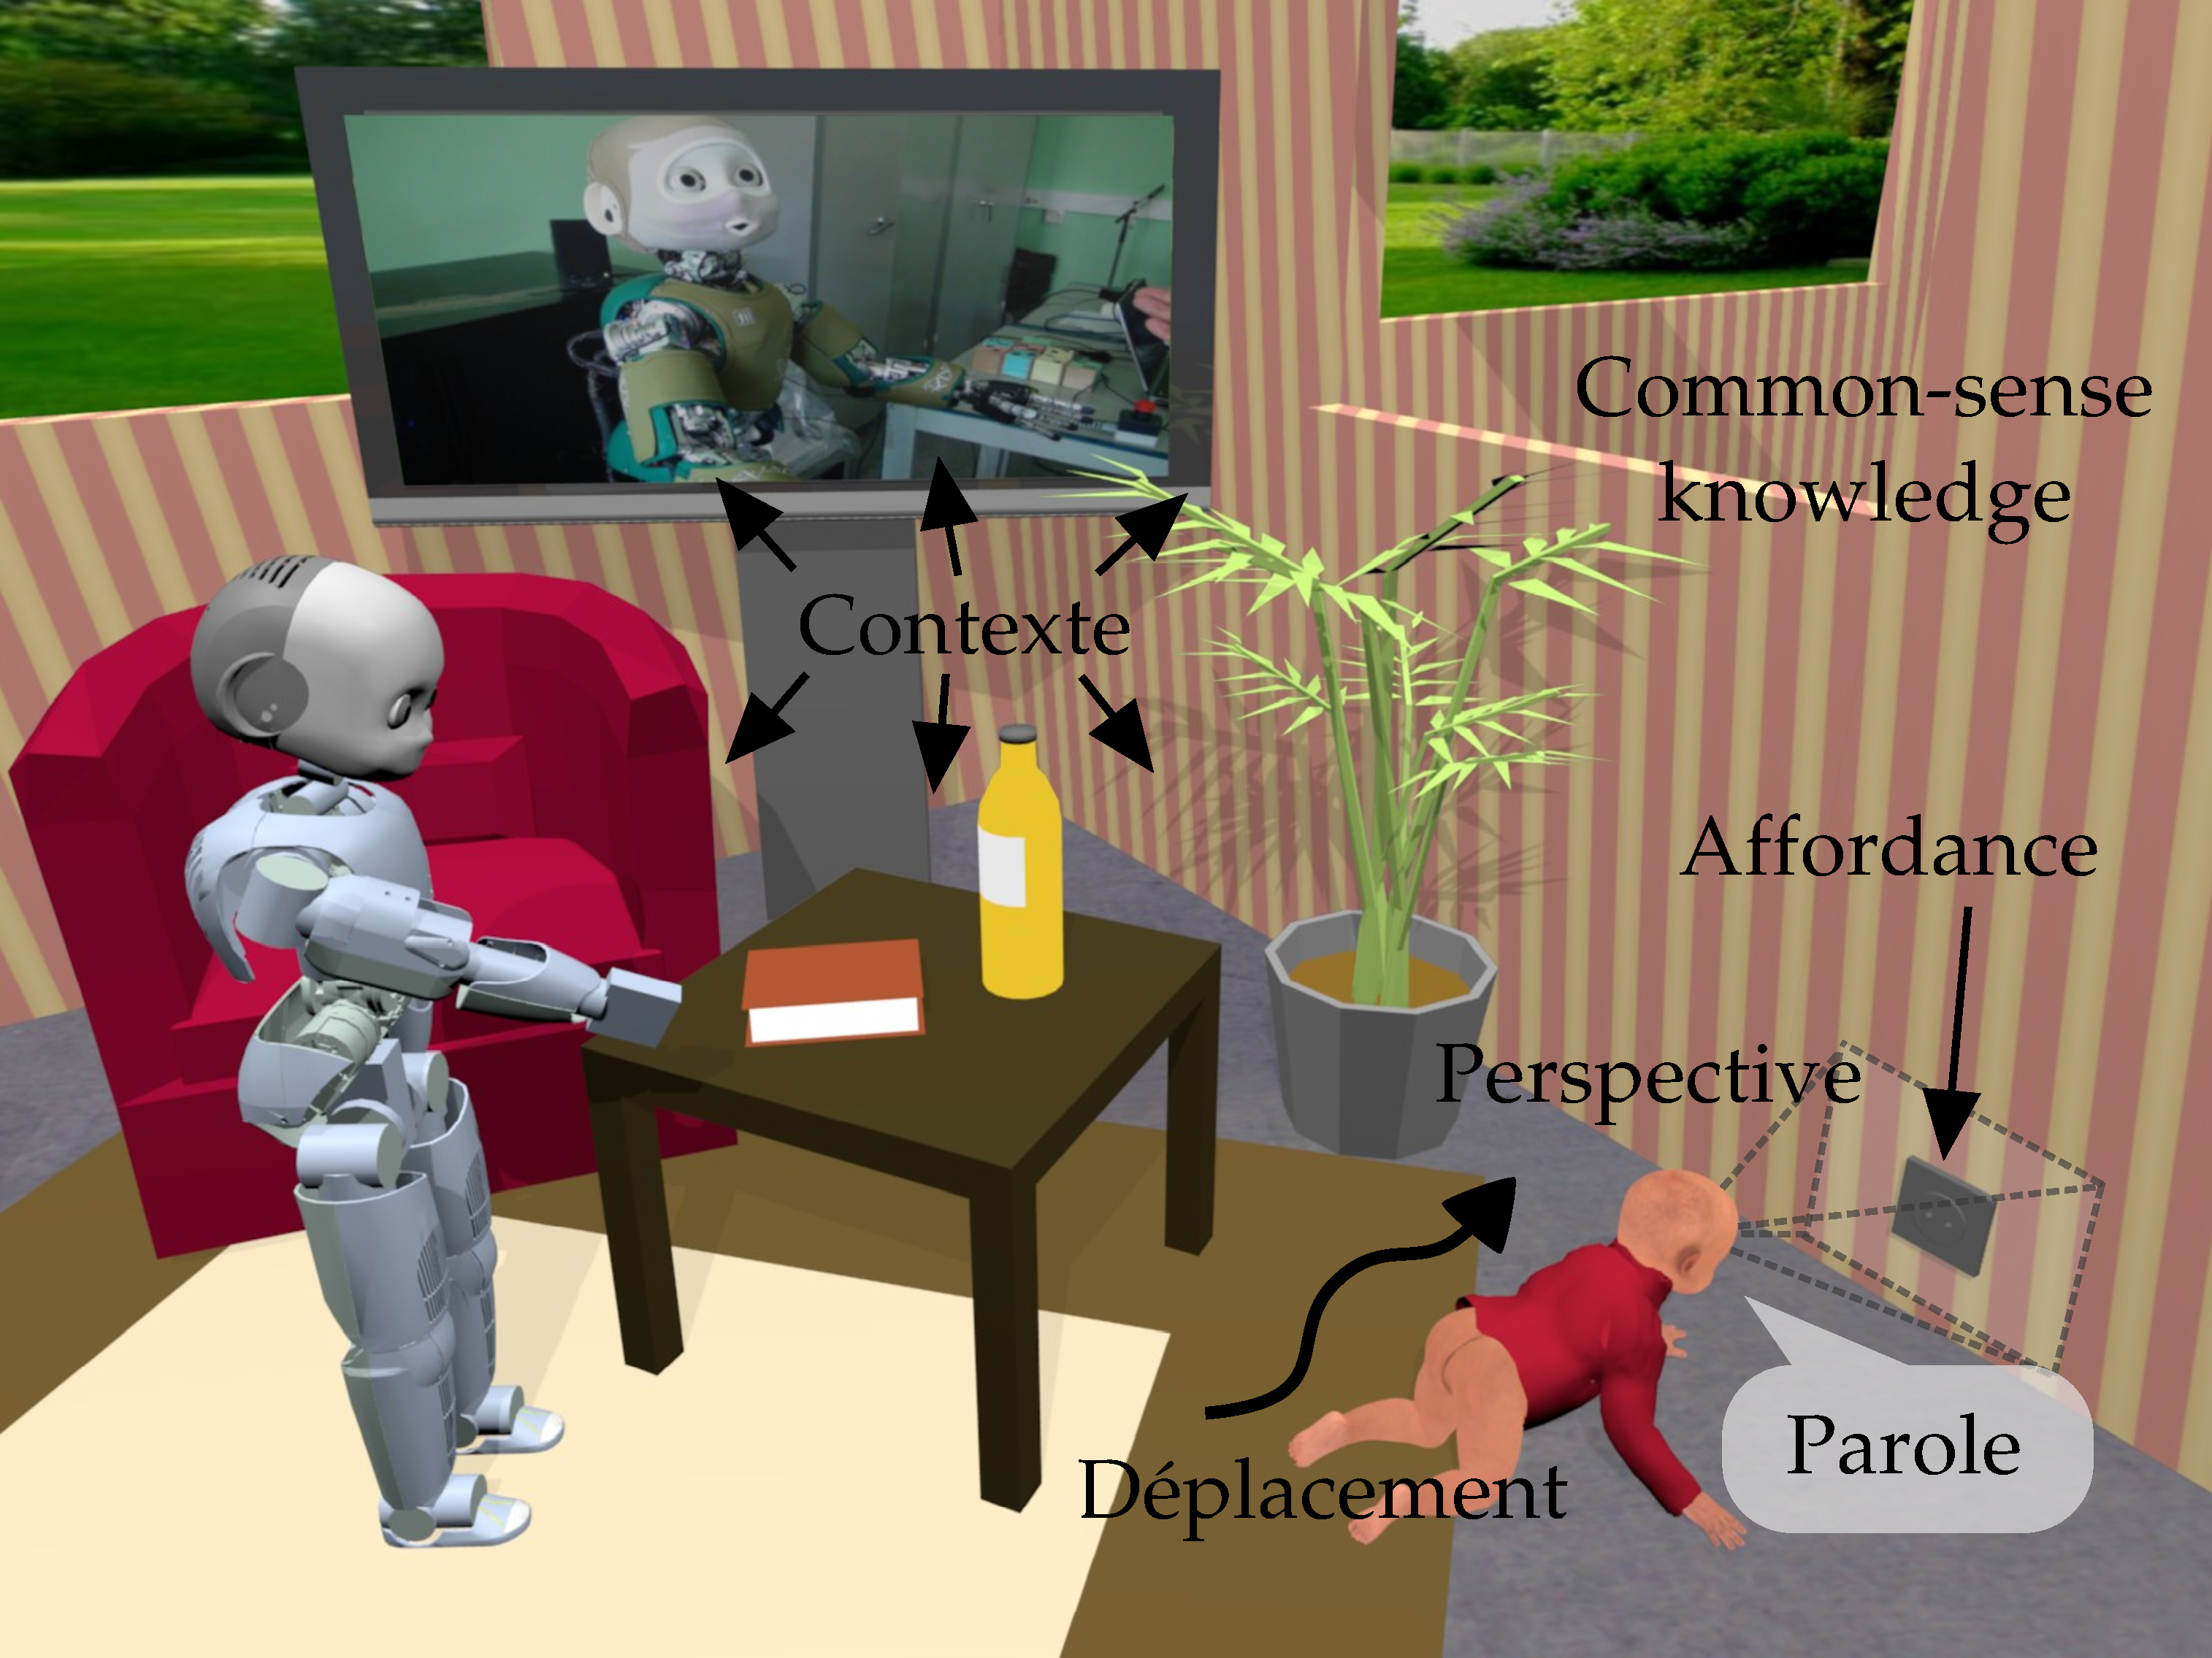
\includegraphics[width=0.8\textwidth]{figs/signaux}
\caption{\small Un robot reconnait une situation de danger : le bébé se dirige
    vers une prise électrique. Cette interprétation nécessite une représentation
    \emph{unifiée} de l'environnement, incluant (a) un modèle géométrique et
    temporel, (b) un modèle des croyances de l'humain construit à partir des
    signaux qu'il émet (déplacement, parole...) et de prise de perspective, (c)
    un modèle sémantique qui inclue une représentation des affordances de
    l'environnement, une représentation du contexte et un modèle du
    \emph{common-sense} (ici par exemple ``une prise est dangereuse'').}

\label{babyplug}
\end{figure}

Le deuxième axe de recherche s'intéresse à l'utilisation effective, en robotique
cognitive, de cette approche continue, du signal au symbole sémantique. Il
s'intéresse d'abord à la question de la représentation \emph{unifiée} des
différentes modalités, ensuite à l'application de cette représentation pour
implémenter de nouvelles compétences cognitives supérieures chez les robots.

\paragraph{Systèmes de représentation}

L'état de l'art dans le domaine des systèmes de représentation d'environnement
pour les robots est divisé entre les systèmes géométriques/symboliques
(typiquement \emph{amodaux}, et utilisés par l'essentiel des systèmes robotiques
autonomes de haut-niveau, type robotique de service ou robotique d'extérieure),
les approches ancrées (typiquement \emph{modales}), et un certain nombre de
techniques mixtes. Dans la continuité de l'Axe 1, je souhaite rechercher et
introduire un nouveau modèle de l'environnement qui \textbf{unifie} ces
techniques, en s'appuyant sur l'idée d'un \textbf{ensemble de mondes
indépendants}, conjuguant perception ancrée et modélisation symbolique et amodale.

Les recherches actuelles sont essentiellement focalisées sur la représentation
géométrique de l'environnement du robot. La construction en ligne de cartes
sémantiques~\cite{Nuechter2008, Galindo2008, Blodow2011} ou l'utilisation
d'affordances fonctionnelles~\cite{Varadarajan2011} sont des exemples de l'état
de l'art au regard de la construction de liens géométrique-symbolique sur
l'environnement spatial du robot. Ceci débouche sur des représentations
\emph{amodales} (plusieurs modalités sont abstraites dans une représentation
commune) de l'environnement, prenant parfois en compte les incertitudes, voire
permettant de représenter des entités spatiales non-vues~\cite{Mavridis2006}.

La représentation symbolique de l'environnement temporel du robot a aussi fait
l'objet de recherches (avec les idées de \emph{chroniques}~\cite{Ghallab1996},
les logiques temporelles comme la \emph{Linear Temporal Logic}, ou encore
l'idée d'\emph{instantanés}~\cite{Mavridis2006}).  La possibilité de se projeter
naturellement dans les états antérieurs du robot, ou de créer et de représenter
des états futurs hypothétiques n'est cependant pas intégrée au niveau d'une
représentation globale de l'environnement du robot.

Quant à l'intégration de la représentation symbolique d'affordances, de
contextes (comme illustré dans la figure~\ref{babyplug}), de modèles de
croyances et d'intentions, le travail reste largement à faire (on peut toutefois
mentionner la représentation de différentes perspectives, comme
dans~\cite{ros2010which}). Le premier de ces défis étant d'ailleurs de concevoir
une représentation pour les affordances, contextes, croyances qui
puisse être unifiée dans un modèle de l'environnement.

À l'opposé, les approches développementales traitent la question de la
représentation de l'environnement de manière modale : chaque modalité existe en
tant que telle, et les interactions entre modalités sont découverte et apprise
par le système au sein de boucle sensori-motrices. Cependant, comme souligné
par Pezzulo~\cite{pezzulo2012computational}, l'organisation de ces interactions
pour alimenter des processus cognitifs abstraits reste essentiellement une
question ouverte.

[TBD: DyKnow, CAST...]

\begin{figure}
    \centering
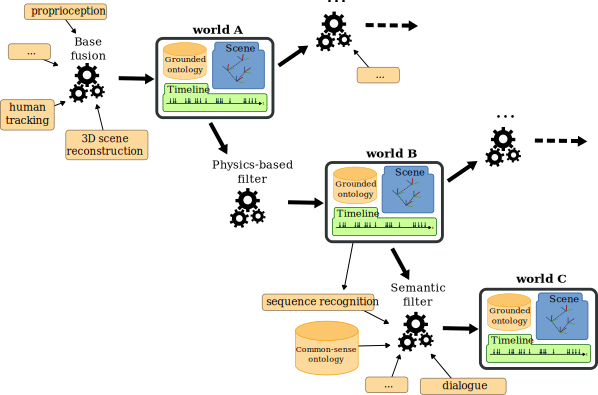
\includegraphics[width=1.0\textwidth]{figs/worlds}
\caption{\small La représentation de l'environnement est envisagée sous la forme
    de mondes (\emph{world A, B, C...}) qui évoluent de manière indépendante les
    uns des autres. Chaque monde a son propre historique (\emph{timeline}), sa
    propre géométrie (\emph{scene}) et son propre modèle cognitif ancré
    (\emph{grounded ontology}).  Les mondes dérivent les uns des autres par des
    transformations (\emph{filters}) successives qui sont alimentées par la
    perception et les connaissances du robot.  }

\label{worlds}
\end{figure}

Intégrer et unifier ces différentes représentations nécessite de largement
repenser les approches actuelles. La figure~\ref{worlds} illustre les premiers
éléments d'une nouvelle proposition allant dans ce sens, que j'ai prototypé en
post-doctorat. Il s'agit d'un paradigme de représentation de l'environnement
basé sur l'idée de \textbf{mondes} existant et évoluant indépendamment et
pouvant représenter des facettes différentes de la réalité du robot, comme un
état futur hypothétique, l'état du monde tel que perçu par un autre agent,
etc. Ces mondes dérivent les uns des autres via des \textbf{filtres cognitifs}
(similaires aux \emph{zones de convergences} suggérées par
Damasio~\cite{damasio1989time} en neurosciences). Ces filtres sont construits
sur les mécanismes de perception à disposition du robot ou sur d'autres sources de
connaissance (comme le modèle physique de l'environnement, ou des connaissances
symboliques \textit{a priori} sur tel ou tel objet).

J'ai initialement conçu ce paradigme à partir des besoins, identifiés durant
mon doctorat au LAAS, des superviseurs de robot d'interaction : je veux
approfondir cette approche pour y intégrer en profondeur les techniques
présentées dans l'Axe 1, et valider ensuite ce modèle de représentation sur le
terrain, comme présenté ci-après, dans la section Programme Expérimental.

\paragraph{Modélisation mutuelle homme-robot}


Je propose de construire cette recherche sur les représentations en robotique
autour du domaine particulier de la \textbf{modélisation mutuelle homme-robot} :
les dynamiques sociales humaines s'appuient sur la capacité à attribuer de
manière pertinente des croyances, des buts et des percepts aux autres. Cet
ensemble de capacités meta-représentationelles forment ce qu'on appelle une
théorie de l'esprit, et conduit à la modélisation mutuelle : la capacité
réciproque d'établir un modèle mental de l'autre. Ceci se retrouve au c\oe ur
des interactions humaines : une interaction sociale normale dépend de la
reconnaissance de perspectives sensorielles différentes, de la compréhension
d'états mentaux différents, et de la reconnaissance d'indices attentionels et
émotionels non-verbaux complexes.  Ce mélange complexe de signal humain et
social, et de modélisation sémantique constitue un défi qui fait de la
modélisation mutuelle un bon champ d'application pour traiter la question de la
représentation de l'environnement du robot.

Ce champ d'application est intéressant à d'autres titres : d'un point de vue
technique, il requiert des approches très multi-modales (chaque modalités venant
enrichir le modèle) et exige une perception fine et rapide pour reconnaitre des
signaux humains subtils ; d'un point de vue scientifique, il fait partie des
sujets qui focalisent actuellement l'attention de la communauté, se situe à un
carrefour disciplinaire particulièrement intéressant, entre psychologie,
robotique et intelligence artificielle, et il représente une compétence
socio-cognitive humaine complexe dont une implémentation générique serait une
avancée notable de l'état de l'art.

Jusqu'à présent, la communauté de l'interaction homme-machine n'a qu'effleuré
cette question : Scassellati donnait en 2002 dans~\cite{scassellati2002theory}
un premier aperçu de la construction d'une théorie de l'esprit du point de vue
de la robotique, sans réelle implémentation. Depuis, la recherche dans ce
domaine s'est essentiellement focalisée sur des applications de prise de
perspective (``\emph{je vois que tu vois la prise}''), utilisant la
vision comme principale (souvent unique) modalité sensorielle. Les principaux
travaux sur cette questions sont par Breazeal~\cite{breazeal2006using},
Trafton~\cite{Trafton2005} et Ros~\cite{Ros2010} (j'ai étroitement travaillé
avec cette dernière sur ces questions).

\begin{figure}[h!t]
        \centering
        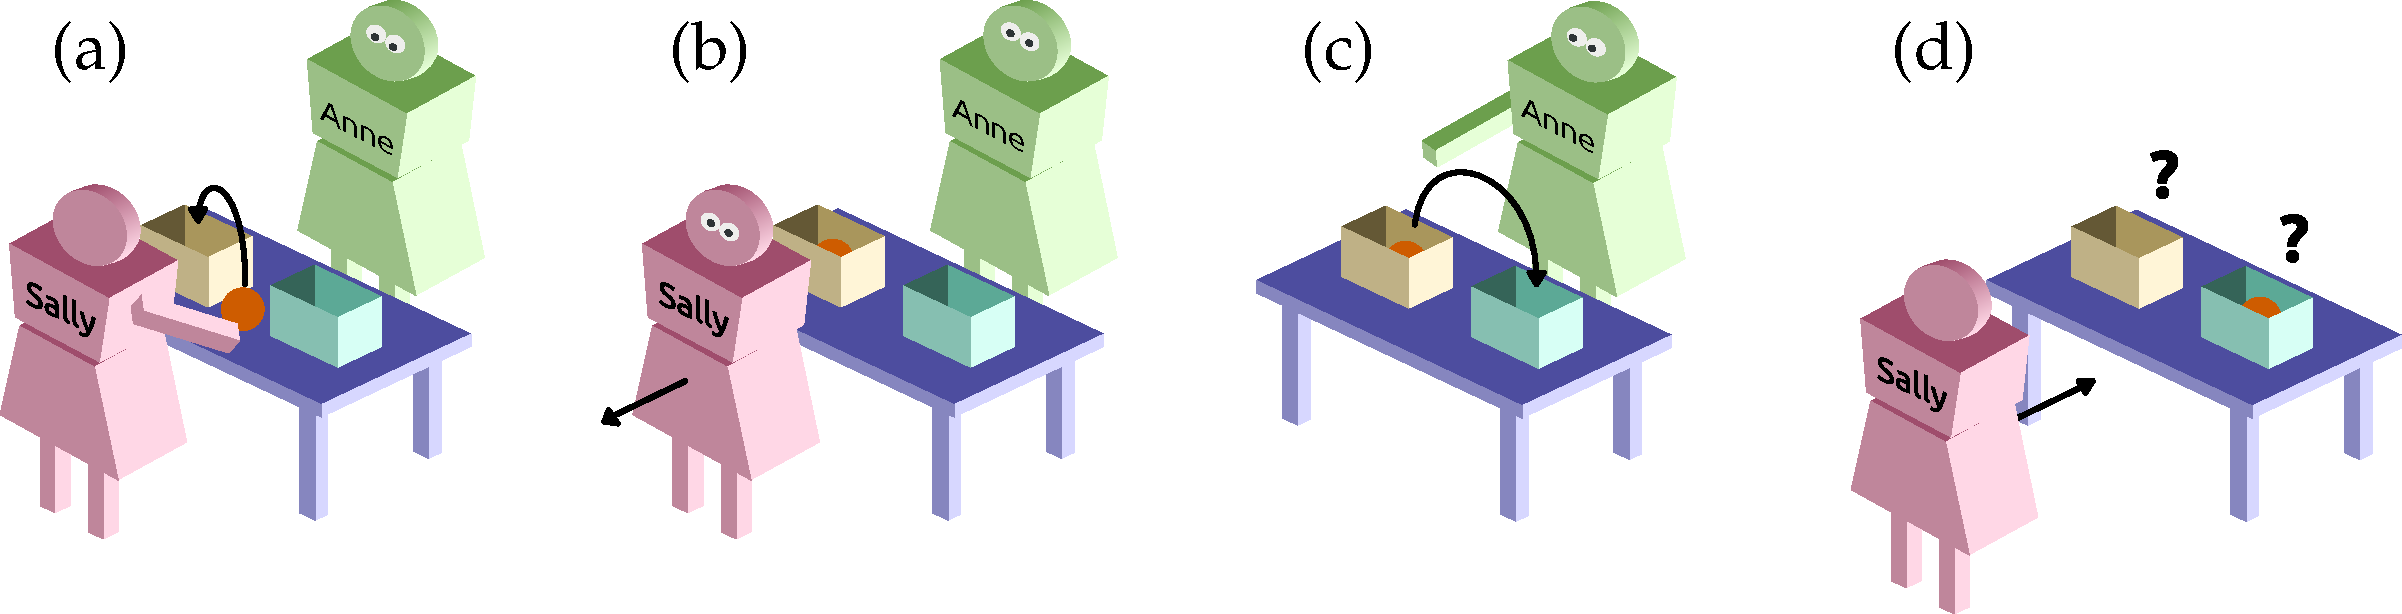
\includegraphics[width=1.0\linewidth]{sally_ann}
        \caption{\small L'expérience de ``False belief'': deux poupées, Anne
            et Sally, se font face, avec deux boites entre elles. Un enfant
            (le sujet) observe la scène. Sally place une balle dans la boite
            beige, puis s'en va. Anne déplace la balle dans la boite bleue, puis
            Sally revient. L'expérimentateur demande à l'enfant: \emph{Où
            penses-tu que Sally va aller chercher la balle ?}. Sans une théorie
            de l'esprit (\ie, avant 3-4 ans), l'enfant n'est pas capable de
            projeter des croyances fausses dans le modèle mental de Sally, et se
            trompe en répondant \emph{Dans la boite bleue}. En terme de
            représentations, une prise de perspective visuelle suffit pour
            réussir cette tâche.}
        \label{false-beliefs}
\end{figure}

En se basant sur une prise de perspective uniquement visuelle, Breazeal
\etal\cite{breazeal2009embodied} et Warnier \etal\cite{warnier2012when} (travail
auquel j'ai également largement participé) ont pu implémenter le test classique de théorie de
l'esprit, l'expérience de Sally et Anne (figure~\ref{false-beliefs}). Ils ont pu
faire la démonstration de systèmes complets dans lesquels le robot reconnait et
prend en compte des situations de croyances fausses et met en \oe uvre des
comportements permettant d'aider le partenaire humain en fonction des
connaissances manquantes ou fausses de celui-ci.

Un travail considérable reste à mener pour généraliser ces résultats au-delà de
percepts visuels simples (``je vois que tu vois...'').
J'ai ébauché dans~\cite{lemaignan2015mutual} un certain nombre de pistes (issues
de la psychologie expérimentale, de la communauté du \emph{Collaborative
Learning} et de l'épistémologie formelle) pour avancer dans cette direction.
L'apport d'un système de représentation unifiant signaux et symboles est l'un
des points clés pouvant effectivement permettre un progrès significatif de
l'état de l'art dans ce domaine.

[A DEVELOPPER: dire ce que je compte faire]

\subsection*{Axe 3 -- Décision distribuée et architecture cognitive pour l'interaction homme-robot}

Comme souligné par Kurup~\cite{kurup2012what}, les compétences cognitives des
robots actuels sont la plupart du temps implémentées et testées indépendamment
les unes des autres et ce n'est que récemment que la robotique s'intéresse aux
architectures cognitives holistiques développées en intelligence artificielle.
Les travaux de Chen~\cite{Chen2010}, de Beetz~\etal~\cite{Beetz2010}, de
Trafton~\etal sur ACT-R/E~\cite{trafton2013act} et les travaux auxquels j'ai
participé au LAAS-CNRS~\cite{lemaignan2014human} en sont parmi les principaux
exemples récents. Ces architectures adoptent toutes une approche symbolique,
dans laquelle les perceptions sont explicitement transformées en objets
symboliques abstraits (typiquement, des formules de logique du premier ordre),
avec lesquels les processus décisionnels travaillent. J'ai montré en particulier
durant mon doctorat qu'il était possible de construire et d'exploiter en ligne
des modèles cognitifs riches des autres agents, et d'intégrer ces modèles dans
la prise de décision~\cite{alami2011when, warnier2012when, lemaignan2014human}.
Pour autant, ces approches ne répondent pas de manière satisfaisante à la
réalité d'une interaction dynamique : la réactivité des robots d'interaction est
aujourd'hui clairement limitée par la complexité et la lenteur des mécanismes
décisionnels en jeu (nécessitant typiquement raisonnement et planification).

En parallèle, un second courant de recherche, animé en particulier par
l'université de Plymouth (Cangelosi, Belpaeme~\etal), propose de considérer les
architectures cognitives à travers une approche
ancrée, s'appuyant sur des réseaux de neurones~\cite{morse2010epigenetic,
baxter2013cognitive}. Ils montrent qu'un certain nombre de fonctions cognitives
haut-niveau peuvent émerger ainsi, comme le phénomène d'alignement
comportemental entre partenaires d'une interaction.
Sans parler d'architecture décisionnelle à proprement parler, plusieurs autres
approches développementales s'intéressent à l'apprentissage de la prise de
décision, notamment l'équipe de Bailly~\cite{mihoub2014modeling} : leur approche
consiste à utiliser un meta-HMM pour reconnaitre différentes situations
d'interaction, et simultanément générer les actions adaptées à ces situations.

\begin{figure}
    \centering
    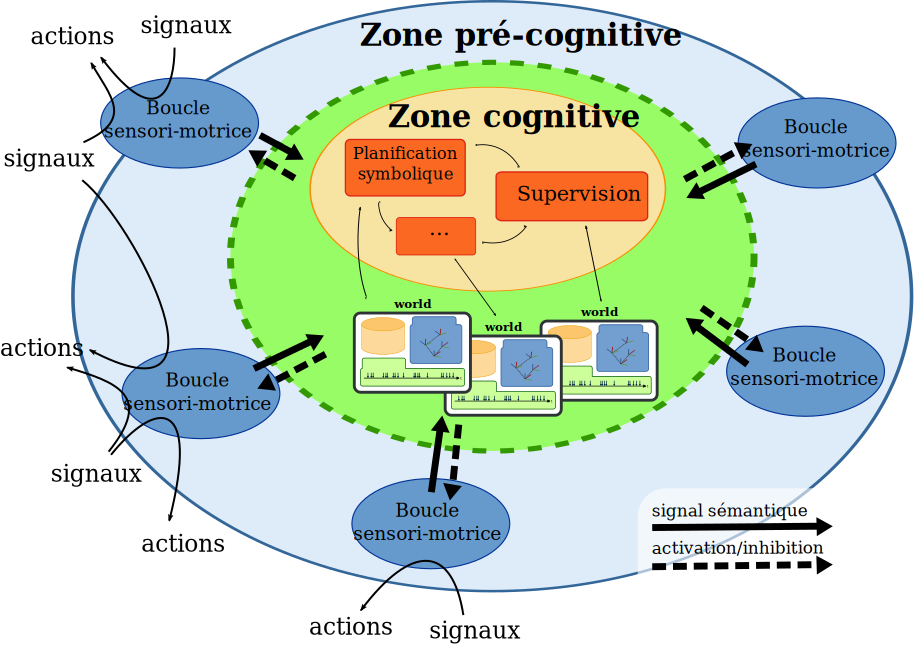
\includegraphics[width=0.7\linewidth]{archi}
    \caption{\small Intégrer un contrôle cognitif explicite avec des boucles
        sensori-motrices ``réflexes'', dites \emph{pré-cognitives}, au sein
    d'un nouveau type d'architecture cognitive pour les robots d'interaction.}
    \label{archi}
\end{figure}

Le troisième axe de recherche que je propose de développer s'intéresse à
l'unification des techniques décisionnelles en robotique. Je propose à cette fin
d'explorer une nouvelle architecture semi-distribuée (figure~\ref{archi}) dans
laquelle un composant symbolique interagit avec un ensemble de boucle
sensori-motrice de manière faiblement couplée, à travers des mécanismes
d'activation/inhibition.

[A DEVELOPPER]

Je souhaite ici aussi valider cette approche en confrontant spécifiquement cette
architecture au domaine de l'interaction homme-robot qui synthétise beaucoup des
défis de la robotique : environnements dynamiques dont la sémantique est
complexe, suivi et représentation de l'homme, action conjointe, nécessité d'une
grande réactivité et d'un parallélisme fort pour assurer une interaction de
qualité.

\subsection*{Programme expérimental}

En me basant sur mon expérience acquise dans la menée d'expérience d'interaction
homme-robot en environnements écologiques et sur des plateformes allant du Nao
au PR2 en passant par
l'iCub~\cite{lemaignan2010oro,ros2010which,lallee2011towards,lemaignan2012roboscopie,warnier2012when,hood2015when},
je propose de matérialiser les axes de recherche que j'ai présenté sous la forme
de plusieurs objectifs expérimentaux, à la fois en laboratoire et sur le
terrain.  Une première série d'expériences vise à démontrer l'intérêt d'une
représentation unifiée de l'environnement du robot pour développer des capacités
cognitives nouvelles ; une seconde série d'expériences s'intéresse à la mise en
place d'une plateforme rigoureuse pour l'expérimentation sur le terrain, et à
son utilisation pour démontrer ces capacités nouvelles dans des scénarios
d'interactions complets en environnement humain naturel. Ce programme
expérimental vise à faire avancer significativement l'état de l'art en ce qui
concerne la robotique d'interaction, aussi bien en termes algorithmiques, qu'en
terme d'intégration concrète et d'usages en situation réelle.

Je propose dans un premier temps de recréer en laboratoire un ensemble de
situations d'interaction dans l'esprit de la figure~\ref{babyplug}: de court
(environ 10 min) épisodes de la vie courante, rigoureusement définis pour former
un benchmark reproductible, et impliquant robots et humains dans des tâches
réalistes de reconnaissance de situation et de manipulation d'objets. Pour ces
scénarios, une interprétation correcte nécessite typiquement de combiner
représentations multi-modales ancrées et représentations sémantiques, d'être
capable de construire un modèle fin de l'homme (incluant la reconnaissance de
séquences d'actions), et de reconnaitre et mobiliser l'ensemble des contextes de
l'interaction (Axes 1 et 2). La qualité et la pertinence des modèles et de
l'interprétation de la scène réalisée par le robot sera ensuite évalué en les
confrontant aux interprétations produites par des observateurs humains placés
dans le même contexte.

Je prévois ensuite une famille d'expériences s'intéressant à une théorie de
l'esprit au niveau des \emph{représentations} (Axe 2) : il s'agit de tester la
capacité du robot à construire un modèle des représentations \emph{abstraites}
des autres (comme je le présente dans~\cite{lemaignan2015mutual}), et je propose
d'explorer cette question à travers l'idée de \emph{tromperie adaptative} : dans
une séquence de jeu, le robot à la possibilité de \emph{mentir} (\ie, de tromper
son partenaire) afin de renouveler l'intérêt ludique et de maintenir
l'engagement de l'autre joueur. Le choix de mentir à un instant donné se base sur
la représentation, estimée par le robot, qu'à le joueur de la situation
courante. Le protocole du \emph{Penny Hiding Game}~\cite{oswald1989role}, issu
de la psychologie expérimentale, met en évidence ces mécanismes : un joueur
cache dans une main un objet, et l'autre joueur doit deviner la main.  Après
quelques essais, des stratégies de jeu se mettent en place pour tromper
l'adversaire et l'inciter à choisir la main incorrecte. Dans un tel scénario,
que je propose d'implémenter sur une plateforme robotique type iCub, le robot
peut adapter cette stratégie de jeu en fonction de ce qu'il perçoit du
comportement, et indirectement, des représentations, de l'autre joueur.

En parallèle de ces expériences de laboratoire ``in vitro'', je souhaite
\textbf{concevoir et mettre en place une plateforme expérimentale ``in vivo''}
pour mener des expériences d'interaction homme-robot sur le terrain. Cette
plateforme aura un axe méthodologique (développement de techniques non-invasives
de mesure de l'engagement humain et de la perception des robots par les humains,
comme j'ai exploré
dans~\cite{lemaignan2014dynamics,lemaignan2014cognitive,fink2014dynamics,sharma2015measuring})
et un axe technologique (en particulier en terme d'architecture logicielle
robuste pour l'interaction, dans la lignée du travail que j'ai mené sur cette
question~\cite{lemaignan2014human,lemaignan2015pyrobots}).

Les expériences que je planifie une fois cette plateforme en place s'intéressent
à la fois au déploiement d'une architecture cognitive pour l'interaction en
autonomie, et aux facteurs cognitifs d'une interaction de longue durée.
L'objectif est typiquement de déployer dans une première phase des robots de
type Nao avec des schémas d'interaction restant simples (tâches du type lecture
de recette ou d'histoire pour les enfants) dans des familles non-expertes, et
sur des périodes longues (de l'ordre de 3 mois), et dans une seconde phase, de
déployer un robot complexe type PR2/iCub dans une famille, pour une durée
longue, et avec un répertoire d'interactions étendu, incluant autonomie
complète, dialogue multi-modal, manipulation conjointe. Je situe cet objectif
expérimental à un horizon J+3 ans.

\subsection*{Conclusion, impact et laboratoire d'accueil}

Je propose dans ce projet trois axes : la recherche de
\textbf{techniques nouvelles permettant de lier signal bas-niveau et modèle
sémantique} ; la conception d'un \textbf{système de représentation unifié,
autour de l'idée d'ontologie multi-modale ancrée} ; la transposition de ces
techniques à la \textbf{décision en robotique, avec la recherche d'une nouvelle
génération d'architectures décisionnelles duales et semi-distribuées}.

Ensemble, ils constituent un ensemble ambitieux, qui :
\begin{itemize}
    \item cherche à \textbf{unifier deux approches scientifiques majeures} en robotique
        cognitive ;
    \item englobe et \textbf{structure un champ large de techniques} issues du \emph{machine
        learning}, de l'intelligence artificielle et du web sémantique pour
        les mettre au service de la robotique ;
    \item a un \textbf{potentiel disruptif} en terme de capacités de représentation, de
        compréhension et d'autonomie pour la robotique ;
    \item se situe à un \textbf{carrefour interdisciplinaire remarquable}, entre
        techniques avancées de traitement de signal complexe, intelligence
        artificielle et sciences cognitives.
\end{itemize}

Le développement de ces axes est par ailleurs soutenu par \textbf{un programme
expérimental fort} qui donne à ces recherches légitimité et impact, y compris au
niveau de la société civile.

Ce programme de recherche mêle étroitement robots et humains. Bien que mise en
avant de manière répétée dans les orientations scientifiques européennes (au
sein des \emph{Future and Emerging Technologies}, les technologies
cognitives sont une des priorités affichées de l'agenda Horizon2020), la
robotique cognitive est relativement peu représentée dans le paysage
scientifique français, les principales équipes de dimensions internationales
étant Flowers, à l'INRIA, et les laboratoires LAAS et ISIR au sein du CNRS. Je
souhaiterais cependant, en premier choix, rejoindre le GIPSA Lab à Grenoble.
Nouveau venu dans le domaine de la robotique, mais de réputation internationale
dans le domaine de l'acquisition et du traitement du signal humain (en
particulier de la parole), il me semble être un environnement remarquable pour
faire progresser la recherche en interaction homme-robot avec des approches
nouvelles et disruptives. Le laboratoire a de plus récemment acquis un robot
iCub, parfaitement adapté à la recherche en interaction homme-robot, et prend
depuis peu une orientation résolument ``robotique cognitive'', comme le traduit
le nouveau nom de l'équipe MAGIC, désormais CRISSP: ``Cognitive Robotics,
Interactive Systems and Speech Processing''.  L'expertise en robotique
d'interaction que je suis susceptible d'apporter s'inscrirait tout à fait dans
cette dynamique.

De plus, d'autres équipes du GIPSA Lab comme l'équipe PCMD (\emph{Parole
Cerveau Multimodalité Développement}) sont spécialistes en cognition et en
psychologie expérimentale, et représentent à ce titre un atout supplémentaire et
renforcent l'intérêt de ce laboratoire pour mener mon programme de recherche.

\printbibliography

\end{document}
